\documentclass[11pt]{article}
\usepackage{sbc-template}
\usepackage{graphicx,url}
\usepackage[utf8]{inputenc}
\usepackage[brazil]{babel}
\usepackage{amsmath,amssymb}
\usepackage{newtxtext}
\usepackage{lmodern}
\usepackage{algorithm}
\usepackage{algpseudocode}
\usepackage{indentfirst}
\usepackage{hyperref}
\usepackage{tikz}
\usepackage{forest}
\usepackage{multicol}
\usepackage{caption}
\sloppy

\title{Aprendizado de Máquina em Sinais Vitais: Modelagem Simbólica e Neural}

\author{Lucas Yukio Fukuda Matsumoto\inst{1}}

\address{Engenharia de Computação -- CSI30 S73 Sistemas Inteligentes\\
Universidade Tecnológica Federal do Paraná (UTFPR) -- Curitiba -- PR -- Brazil\\
\email{lucmat@alunos.utfpr.edu.br}}

\begin{document}
\fontsize{11pt}{11pt}\selectfont
\maketitle

\begin{resumo}
Este artigo apresenta uma análise comparativa entre três abordagens de Aprendizado de Máquina aplicadas ao cenário de sinais vitais: Random Forest Simbólico, C4.5 e Perceptron Multicamadas (MLP). São discutidos os requisitos funcionais e não-funcionais, metodologia, resultados experimentais e impactos éticos e sociais da aplicação dessas técnicas em contextos envolvendo humanos. Os experimentos utilizam um conjunto de dados realista de sinais vitais, e as métricas de avaliação incluem acurácia, RMSE, precisão, recall, F1-score e matriz de confusão. O artigo segue o formato SBC e inclui reflexões sobre privacidade, justiça e confiança nos sistemas inteligentes.
\end{resumo}

\begin{abstract}
This paper presents a comparative analysis of three Machine Learning approaches applied to vital signs: Symbolic Random Forest, C4.5, and Multilayer Perceptron (MLP). We discuss functional and non-functional requirements, methodology, experimental results, and ethical and social impacts of applying these techniques in human-related contexts. Experiments use a realistic vital signs dataset, and evaluation metrics include accuracy, RMSE, precision, recall, F1-score, and confusion matrix. The article follows the SBC format and includes reflections on privacy, fairness, and trust in intelligent systems.
\end{abstract}

\section{Introdução}
O monitoramento de sinais vitais é fundamental em ambientes clínicos e de saúde, permitindo a detecção precoce de anomalias e suporte à tomada de decisão médica~\cite{clifford2012advanced}. Com o avanço da Aprendizagem de Máquina (AM), tornou-se possível modelar padrões complexos em dados biomédicos, promovendo diagnósticos mais precisos e automação de processos~\cite{shickel2017deep}. Além disso, questões como privacidade, justiça e explicabilidade têm ganhado destaque na literatura recente~\cite{mehrabi2021survey,voigt2017gdpr}. Este artigo explora três modelagens distintas de AM aplicadas a sinais vitais: Random Forest Simbólico, C4.5 e Perceptron Multicamadas (MLP), avaliando suas características, desempenho e impactos sociais.

\section{Objetivo da Tarefa}
O objetivo desta tarefa é reconstruir, por meio de técnicas de aprendizado de máquina, a fórmula de cálculo da gravidade do estado de saúde de vítimas de acidentes (regressão) e a classificação em quatro categorias de gravidade (classificação), a partir de sinais vitais históricos. A motivação é a perda da fórmula original e dos intervalos de classificação definidos por especialistas, exigindo a aplicação de modelos capazes de inferir tanto o valor contínuo da gravidade quanto a classe correspondente. O contexto é o resgate de vítimas em catástrofes naturais, desastres ou grandes acidentes, onde decisões rápidas e precisas são essenciais.

\section{Fundamentação Teórica}
\subsection{Sinais Vitais e Ciência de Dados}
Sinais vitais são indicadores fisiológicos essenciais para o monitoramento do estado de saúde de pacientes, incluindo frequência cardíaca, pressão arterial, temperatura corporal e saturação de oxigênio~\cite{clifford2012advanced}. A análise automatizada desses sinais, por meio de técnicas de ciência de dados, permite identificar padrões e anomalias que podem não ser perceptíveis a olho nu, contribuindo para diagnósticos mais rápidos e precisos.

\subsection{Aprendizagem de Máquina em Saúde}
A aplicação de AM em saúde tem crescido exponencialmente, com destaque para o uso de redes neurais profundas em registros eletrônicos de saúde (EHR)~\cite{shickel2017deep}. Modelos supervisionados, como árvores de decisão e redes neurais, são amplamente utilizados para tarefas de classificação e regressão em dados biomédicos, proporcionando avanços significativos em predição e suporte à decisão clínica.

\subsection{Árvores de Decisão e C4.5}
O algoritmo C4.5, proposto por Quinlan~\cite{quinlan1993c4.5}, é uma evolução do ID3 e utiliza o ganho de informação normalizado (gain ratio) para selecionar atributos, além de suportar atributos contínuos e realizar poda para evitar overfitting. Árvores de decisão são valorizadas por sua interpretabilidade, permitindo a extração de regras explícitas a partir dos dados.

\textbf{Formalismo Matemático:}
\begin{itemize}
    \item \textbf{Entropia:}
    \[
    H(S) = -\sum_{i=1}^k p_i \log_2 p_i
    \]
    Onde:
    \begin{itemize}
        \item $H(S)$: entropia do conjunto $S$;
        \item $S$: conjunto de exemplos;
        \item $k$: número de classes;
        \item $p_i$: proporção de exemplos da classe $i$ em $S$.
    \end{itemize}
    Mede a incerteza dos rótulos no conjunto $S$.
    \item \textbf{Ganho de Informação:}
    \[
    IG(S, A) = H(S) - \sum_{v \in \text{Valores}(A)} \frac{|S_v|}{|S|} H(S_v)
    \]
    Onde:
    \begin{itemize}
        \item $IG(S, A)$: ganho de informação do atributo $A$ sobre $S$;
        \item $A$: atributo avaliado;
        \item $v$: valor possível de $A$;
        \item $S_v$: subconjunto de $S$ onde $A = v$;
        \item $|S_v|$: número de exemplos em $S_v$;
        \item $|S|$: número de exemplos em $S$;
        \item $H(S_v)$: entropia do subconjunto $S_v$.
    \end{itemize}
    \item \textbf{Índice de Valor (IV):}
    \[
    IV(A) = -\sum_{v \in \text{Valores}(A)} \frac{|S_v|}{|S|} \log_2 \frac{|S_v|}{|S|}
    \]
    Onde:
    \begin{itemize}
        \item $IV(A)$: índice de valor do atributo $A$;
        \item $v$: valor possível de $A$;
        \item $|S_v|$: número de exemplos em $S_v$;
        \item $|S|$: número de exemplos em $S$.
    \end{itemize}
    \item \textbf{Gain Ratio:}
    \[
    GR(S, A) = \frac{IG(S, A)}{IV(A)}
    \]
    Onde:
    \begin{itemize}
        \item $GR(S, A)$: razão de ganho do atributo $A$ em $S$;
        \item $IG(S, A)$: ganho de informação;
        \item $IV(A)$: índice de valor.
    \end{itemize}
\end{itemize}

\paragraph{Parâmetros do C4.5}
\begin{itemize}
    \item \textbf{max\_depth} (int): Profundidade máxima da árvore. Valores típicos: 1 a 30. Profundidades maiores aumentam a capacidade de ajuste, mas podem causar overfitting.
    \item \textbf{min\_samples\_split} (int): Número mínimo de amostras para dividir um nó. Valores comuns: 2 a 20. Valores maiores tornam a árvore mais conservadora.
    \item \textbf{pruning} (bool): Ativa ou desativa a poda. Poda reduz overfitting, mas pode diminuir levemente a acurácia.
    \item \textbf{criterion} (str): Critério de divisão. Opções: \texttt{gain\_ratio} (padrão), \texttt{entropy}, \texttt{gini}. O \texttt{gain\_ratio} é mais robusto para atributos com muitos valores.
    \item \textbf{random\_state} (int): Semente para reprodutibilidade. Qualquer inteiro.
\end{itemize}

\paragraph{Influência dos Parâmetros}
\begin{itemize}
    \item \textbf{max\_depth}: Profundidades maiores permitem que a árvore capture padrões mais complexos, mas aumentam o risco de overfitting, especialmente em conjuntos de dados pequenos ou ruidosos.
    \item \textbf{min\_samples\_split}: Valores maiores tornam a árvore mais conservadora, reduzindo o risco de overfitting, mas podem diminuir a capacidade de capturar padrões sutis.
    \item \textbf{pruning}: A poda reduz o overfitting ao eliminar ramos pouco relevantes, tornando o modelo mais simples e generalizável, mas pode reduzir levemente a acurácia em alguns casos.
    \item \textbf{criterion}: O critério de divisão afeta a escolha dos atributos nos nós. O \texttt{gain\_ratio} é mais robusto para atributos com muitos valores, enquanto \texttt{entropy} e \texttt{gini} podem ser mais sensíveis a ruídos.
    \item \textbf{random\_state}: Garante reprodutibilidade dos resultados, não afetando o desempenho, mas permitindo comparar execuções.
\end{itemize}

\subsection{Random Forest Simbólico}
O Random Forest tradicional consiste em um conjunto de árvores de decisão treinadas com amostragem bootstrap e seleção aleatória de atributos~\cite{pedregosa2011scikit}. No Random Forest Simbólico, cada árvore é composta por nós que representam operações matemáticas simbólicas.

\textbf{Formalismo Matemático:}
\begin{itemize}
    \item \textbf{Bootstrap:} Para cada árvore $T_j$, sorteia-se uma amostra $D_j$ de $D$ com reposição, onde:
    \begin{itemize}
        \item $T_j$: $j$-ésima árvore do ensemble;
        \item $D$: conjunto de dados original;
        \item $D_j$: amostra bootstrap de $D$ para a árvore $T_j$.
    \end{itemize}
    \item \textbf{Árvore Simbólica:} Cada nó executa uma operação $f(\cdot)$ sobre variáveis de entrada ou saídas de outros nós, onde:
    \begin{itemize}
        \item $f(\cdot)$: função matemática (ex: soma, produto, seno, etc.).
    \end{itemize}
    \item \textbf{Predição do Ensemble:}
    \[
    \hat{y} = \frac{1}{N} \sum_{j=1}^N T_j(x)
    \]
    Onde:
    \begin{itemize}
        \item $\hat{y}$: predição final do ensemble;
        \item $N$: número de árvores no ensemble;
        \item $T_j(x)$: saída da árvore $j$ para a entrada $x$;
        \item $x$: vetor de atributos de entrada.
    \end{itemize}
\end{itemize}

\paragraph{Parâmetros do Random Forest Simbólico}
\begin{itemize}
    \item \textbf{n\_estimators} (int): Número de árvores no ensemble. Valores comuns: 10 a 200. Mais árvores aumentam robustez, mas elevam o custo computacional.
    \item \textbf{max\_depth} (int): Profundidade máxima de cada árvore simbólica. Valores típicos: 2 a 10. Profundidades maiores aumentam a capacidade, mas podem causar overfitting.
    \item \textbf{operations} (list): Lista de operações matemáticas permitidas nos nós internos. Exemplos: \texttt{['+', '-', '*', '/', 'sin', 'log']}. Operações mais complexas aumentam a expressividade, mas podem dificultar a interpretabilidade.
    \item \textbf{random\_state} (int): Semente para reprodutibilidade.
    \item \textbf{bootstrap} (bool): Se True, utiliza amostragem bootstrap. Recomenda-se True para maior diversidade.
    \item \textbf{task} (str): Tipo de tarefa (\texttt{classification} ou \texttt{regression}).
\end{itemize}

\paragraph{Influência dos Parâmetros}
\begin{itemize}
    \item \textbf{n\_estimators}: Um número maior de árvores tende a aumentar a robustez e estabilidade do modelo, reduzindo o risco de overfitting em relação a uma única árvore. No entanto, aumenta o tempo de treinamento e predição.
    \item \textbf{max\_depth}: Profundidades maiores permitem que as árvores capturem relações mais complexas, mas podem levar ao overfitting, especialmente com poucos dados ou dados ruidosos.
    \item \textbf{operations}: Operações matemáticas mais variadas aumentam a capacidade de modelagem simbólica, mas podem dificultar a interpretabilidade e aumentar o risco de overfitting.
    \item \textbf{random\_state}: Garante reprodutibilidade dos resultados. Não afeta desempenho, mas permite comparar execuções.
    \item \textbf{bootstrap}: Ativar aumenta a diversidade entre as árvores, melhorando a generalização do ensemble.
    \item \textbf{task}: Define se o modelo será ajustado para regressão ou classificação, influenciando a função de perda e a forma de agregação das saídas.
\end{itemize}

\subsection{Perceptron Multicamadas (MLP)}
O Perceptron Multicamadas (MLP) é uma arquitetura específica de rede neural artificial composta por múltiplas camadas de perceptrons, proposta por Rumelhart, Hinton e Williams~\cite{rumelhart1986learning}, sendo uma evolução do Perceptron original de Rosenblatt~\cite{rosenblatt1958perceptron}. Diferente do termo genérico "rede neural multicamadas", que pode englobar arquiteturas convolucionais, recorrentes, etc., o MLP refere-se estritamente a redes feedforward totalmente conectadas.

\textbf{Formalismo Matemático:}
\begin{itemize}
    \item \textbf{Camada Linear:}
    \[
    z^{(l)} = W^{(l)} a^{(l-1)} + b^{(l)}
    \]
    Onde:
    \begin{itemize}
        \item $z^{(l)}$: vetor de ativações lineares da camada $l$;
        \item $W^{(l)}$: matriz de pesos da camada $l$;
        \item $a^{(l-1)}$: vetor de ativações da camada anterior ($l-1$);
        \item $b^{(l)}$: vetor de bias da camada $l$.
    \end{itemize}
    \item \textbf{Ativação:}
    \[
    a^{(l)} = \phi(z^{(l)})
    \]
    Onde:
    \begin{itemize}
        \item $a^{(l)}$: vetor de ativações da camada $l$;
        \item $\phi$: função de ativação (ex: ReLU, sigmoide, tanh, swish, gelu, mish, leaky\_relu, elu);
        \item $z^{(l)}$: vetor de ativações lineares da camada $l$.
    \end{itemize}
    \item \textbf{Saída:}
    \[
    y = a^{(L)}
    \]
    Onde:
    \begin{itemize}
        \item $y$: saída da rede;
        \item $a^{(L)}$: ativações da última camada ($L$).
    \end{itemize}
    \item \textbf{Função de Custo (MSE):}
    \[
    J = \frac{1}{n} \sum_{i=1}^n (y_i - \hat{y}_i)^2
    \]
    Onde:
    \begin{itemize}
        \item $J$: valor da função de custo (erro quadrático médio);
        \item $n$: número de exemplos;
        \item $y_i$: valor real do exemplo $i$;
        \item $\hat{y}_i$: valor predito para o exemplo $i$.
    \end{itemize}
    \item \textbf{Backpropagation:}
    \[
    \frac{\partial J}{\partial W^{(l)}} = \delta^{(l)} (a^{(l-1)})^T
    \]
    Onde:
    \begin{itemize}
        \item $\frac{\partial J}{\partial W^{(l)}}$: gradiente da função de custo em relação aos pesos da camada $l$;
        \item $\delta^{(l)}$: vetor de erro propagado na camada $l$;
        \item $a^{(l-1)}$: ativações da camada anterior.
    \end{itemize}
\end{itemize}

\textbf{Formalismo do Perceptron:}
\[
y = \phi\left(\sum_{i=1}^n w_i x_i + b\right)
\]
Onde:
\begin{itemize}
    \item $y$: saída do perceptron;
    \item $w_i$: peso associado à entrada $x_i$;
    \item $x_i$: valor da $i$-ésima entrada;
    \item $b$: bias;
    \item $\phi$: função de ativação.
\end{itemize}

\textbf{Referências históricas:}
\begin{itemize}
    \item Perceptron: Rosenblatt, F. (1958). The Perceptron: A Probabilistic Model for Information Storage and Organization in the Brain~\cite{rosenblatt1958perceptron}.
    \item MLP e retropropagação: Rumelhart, D. E., Hinton, G. E., \& Williams, R. J. (1986). Learning representations by back-propagating errors~\cite{rumelhart1986learning}.
\end{itemize}

\paragraph{Parâmetros do Perceptron Multicamadas (MLP)}
\begin{itemize}
    \item \textbf{input\_dim} (int): Número de atributos de entrada. Deve ser igual ao número de colunas do dataset.
    \item \textbf{output\_dim} (int): Número de saídas (classes ou valor contínuo).
    \item \textbf{hidden\_layers} (list): Lista com o número de neurônios em cada camada oculta, ex: \texttt{[128, 64, 32]}. Mais camadas e neurônios aumentam a capacidade, mas exigem mais dados e regularização.
    \item \textbf{activation} (str): Função de ativação das camadas ocultas. Opções: \texttt{relu}, \texttt{sigmoid}, \texttt{tanh}, \texttt{swish}, \texttt{gelu}, \texttt{mish}, \texttt{leaky\_relu}, \texttt{elu}. Funções não-lineares permitem modelar relações complexas.
    \item \textbf{dropout} (float): Taxa de dropout (0 a 1). Dropout reduz overfitting, mas valores altos podem prejudicar o aprendizado.
    \item \textbf{batch\_norm} (bool): Aplica Batch Normalization após cada camada oculta. Acelera e estabiliza o treinamento.
    \item \textbf{layer\_norm} (bool): Aplica Layer Normalization após cada camada oculta. Útil para redes profundas.
    \item \textbf{lr} (float): Taxa de aprendizado. Valores típicos: $10^{-4}$ a $10^{-2}$. Taxas altas aceleram o treino, mas podem causar instabilidade.
    \item \textbf{batch\_size} (int): Tamanho do batch para SGD. Valores comuns: 16 a 256. Batches maiores tornam o treino mais estável, mas exigem mais memória.
    \item \textbf{epochs} (int): Número máximo de épocas de treinamento. Mais épocas aumentam a chance de convergência, mas podem causar overfitting.
    \item \textbf{patience} (int): Número de épocas sem melhora na validação para acionar o early stopping. Valores típicos: 5 a 20.
    \item \textbf{task} (str): Tipo de tarefa (\texttt{classification} ou \texttt{regression}).
    \item \textbf{verbose} (bool): Exibe logs de treinamento.
\end{itemize}

\paragraph{Influência dos Parâmetros}
\begin{itemize}
    \item \textbf{Mais camadas/neuronios}: aumentam a capacidade de modelagem, mas exigem mais dados e regularização.
    \item \textbf{Função de ativação}: ativações como ReLU aceleram o treino, enquanto sigmoide/tanh podem saturar. Swish, GELU e Mish são modernas e podem melhorar desempenho.
    \item \textbf{Dropout}: reduz overfitting, mas valores altos (acima de 0.5) podem prejudicar o aprendizado.
    \item \textbf{BatchNorm/LayerNorm}: aceleram e estabilizam o treino, especialmente em redes profundas.
    \item \textbf{Taxa de aprendizado}: valores altos podem causar divergência, baixos tornam o treino lento.
    \item \textbf{Batch size}: batches pequenos aumentam ruído, grandes exigem mais memória.
    \item \textbf{Early stopping}: evita overfitting em datasets pequenos.
\end{itemize}

\textbf{Exemplo de configuração:}
\begin{verbatim}
NeuralNetwork(
    input_dim=8,
    output_dim=4,
    hidden_layers=[128, 64, 32],
    activation='swish',
    dropout=0.2,
    batch_norm=True,
    layer_norm=False,
    lr=1e-3,
    batch_size=64,
    epochs=100,
    patience=10,
    task='classification',
    verbose=True
)
\end{verbatim}

\subsection{Métricas de Avaliação}
\begin{itemize}
    \item \textbf{Acurácia:}
    \[
    \mathrm{Acc} = \frac{1}{n} \sum_{i=1}^n \mathbb{I}(y_i = \hat{y}_i)
    \]
    Onde:
    \begin{itemize}
        \item $\mathrm{Acc}$: acurácia;
        \item $n$: número de exemplos;
        \item $y_i$: valor real do exemplo $i$;
        \item $\hat{y}_i$: valor predito para o exemplo $i$;
        \item $\mathbb{I}$: função indicadora (1 se $y_i = \hat{y}_i$, 0 caso contrário).
    \end{itemize}
    \item \textbf{RMSE:}
    \[
    \mathrm{RMSE} = \sqrt{\frac{1}{n} \sum_{i=1}^n (y_i - \hat{y}_i)^2}
    \]
    Onde:
    \begin{itemize}
        \item $\mathrm{RMSE}$: raiz do erro quadrático médio;
        \item $n$: número de exemplos;
        \item $y_i$: valor real do exemplo $i$;
        \item $\hat{y}_i$: valor predito para o exemplo $i$.
    \end{itemize}
    \item \textbf{Precisão:}
    \[
    \mathrm{Prec} = \frac{TP}{TP + FP}
    \]
    Onde:
    \begin{itemize}
        \item $\mathrm{Prec}$: precisão;
        \item $TP$: verdadeiros positivos;
        \item $FP$: falsos positivos.
    \end{itemize}
    \item \textbf{Recall:}
    \[
    \mathrm{Rec} = \frac{TP}{TP + FN}
    \]
    Onde:
    \begin{itemize}
        \item $\mathrm{Rec}$: recall (sensibilidade);
        \item $TP$: verdadeiros positivos;
        \item $FN$: falsos negativos.
    \end{itemize}
    \item \textbf{F1-score:}
    \[
    \mathrm{F1} = 2 \cdot \frac{\mathrm{Prec} \cdot \mathrm{Rec}}{\mathrm{Prec} + \mathrm{Rec}}
    \]
    Onde:
    \begin{itemize}
        \item $\mathrm{F1}$: F1-score;
        \item $\mathrm{Prec}$: precisão;
        \item $\mathrm{Rec}$: recall.
    \end{itemize}
    \item \textbf{Matriz de confusão:} Matriz $C$ onde $C_{i,j}$ indica o número de exemplos da classe $i$ classificados como $j$.
\end{itemize}

\section{Bibliotecas Utilizadas}
\begin{itemize}
    \item \textbf{pandas}: Biblioteca para manipulação e análise de dados tabulares. Utilizada para carregar, limpar, alinhar e combinar datasets, além de facilitar operações de pré-processamento.
    \item \textbf{numpy}: Biblioteca para operações matemáticas e manipulação de arrays. Usada para cálculos vetorizados, normalização e operações numéricas eficientes.
    \item \textbf{scikit-learn}: Biblioteca de aprendizado de máquina em Python. Utilizada para validação cruzada, cálculo de métricas (acurácia, RMSE, precisão, recall, F1-score), e como inspiração para a estrutura dos algoritmos implementados.
    \item \textbf{algorithmicx/algorithm/algpseudocode}: Pacotes LaTeX para apresentação de pseudocódigos de algoritmos no apêndice.
    \item \textbf{graphicx}: Inclusão de imagens e gráficos, como a matriz de confusão (no apêndice).
    \item \textbf{amsmath, amssymb}: Notação matemática e símbolos para fórmulas e equações.
    \item \textbf{lmodern, newtxtext}: Fontes modernas para melhor apresentação do texto.
    \item \textbf{hyperref}: Geração de links e navegação no PDF.
    \item \textbf{indentfirst, url, sbc-template}: Formatação e padronização do artigo conforme normas SBC.
    \item \textbf{tikz, forest}: Desenho de diagramas e árvores no apêndice.
\end{itemize}

\section{Metodologia}
\subsection{Descrição do Dataset}
O conjunto de dados utilizado contém registros de sinais vitais de vítimas de acidentes, com atributos como qualidade da pressão arterial (qPA), pulso (batimentos por minuto), frequência respiratória, gravidade (valor contínuo) e classe de gravidade (1=crítico, 2=instável, 3=potencialmente estável, 4=estável). Os dados foram divididos em conjuntos de treino/validação e teste, conforme recomendado em~\cite{pedregosa2011scikit}.

\subsection{Pré-processamento}
Foram aplicadas as seguintes etapas:
\begin{itemize}
    \item Remoção de valores ausentes, utilizando imputação por média ou mediana.
    \item Normalização dos atributos numéricos para a faixa [0,1].
    \item Codificação de rótulos para classificação multiclasse.
    \item Análise exploratória para detecção de outliers e correlação entre atributos.
\end{itemize}
Essas etapas são essenciais para garantir a qualidade dos dados e a robustez dos modelos~\cite{shickel2017deep}.

\subsection{Gerenciamento de Dados e Utilitários}
O gerenciamento dos dados foi realizado pela classe \texttt{DatasetManager}, responsável por carregar, alinhar e combinar diferentes conjuntos de dados. As principais funções são:
\begin{itemize}
    \item \texttt{load\_train\_dataset}: Carrega dados de treino e separa features e rótulos.
    \item \texttt{load\_predict\_dataset}: Carrega dados para predição.
    \item \texttt{combine\_train\_datasets}: Alinha e concatena múltiplos datasets de treino.
    \item \texttt{align\_features}: Garante que os dados de predição tenham as mesmas colunas dos dados de treino.
\end{itemize}
O código utiliza \texttt{pandas} para manipulação eficiente dos dados e suporta tanto tarefas de treino quanto de predição.

\subsection{Estrutura Abstrata dos Modelos}
Todos os modelos implementam a interface abstrata \texttt{Algorithm}, que define métodos essenciais como \texttt{fit}, \texttt{predict}, \texttt{score} e \texttt{is\_fitted}. Isso garante padronização na avaliação e integração dos modelos, facilitando a comparação direta entre diferentes abordagens.

\subsection{Modelos Utilizados}
\subsubsection{Random Forest Simbólico}
Implementação própria baseada em árvores simbólicas, onde cada nó representa operações matemáticas ou variáveis do dataset. O ensemble é formado por múltiplas árvores geradas aleatoriamente, conforme descrito em~\cite{pedregosa2011scikit}. Cada árvore é construída de forma independente, promovendo diversidade no ensemble e aumentando a robustez do modelo. Utilizado tanto para regressão (predição do valor da gravidade) quanto para classificação (classe de gravidade).

\subsubsection{C4.5}
Algoritmo de árvore de decisão que utiliza ganho de informação normalizado (gain ratio) para seleção de atributos, suportando atributos contínuos e poda pós-processamento~\cite{quinlan1993c4.5}. O C4.5 é reconhecido por sua capacidade de gerar regras interpretáveis e por sua eficiência em cenários com muitos atributos. Utilizado para classificação das classes de gravidade.

\subsubsection{Perceptron Multicamadas (MLP)}
A classe \texttt{NeuralNetwork} implementa um Perceptron Multicamadas (MLP) com auxílio do \texttt{numpy}. O MLP é composto por uma camada de entrada, múltiplas camadas ocultas e uma camada de saída. Cada neurônio realiza uma combinação linear dos sinais de entrada, seguida de uma função de ativação não-linear. O treinamento é realizado pelo algoritmo de retropropagação do erro (backpropagation), ajustando os pesos para minimizar a função de perda (MSE para regressão ou entropia cruzada para classificação). O modelo suporta funções de ativação ReLU, sigmoide e tanh, além de regularização via dropout e early stopping. O MLP pode ser utilizado tanto para regressão quanto para classificação multiclasse, sendo flexível para diferentes tarefas biomédicas.

\subsection{Parametrização dos Algoritmos}
\begin{itemize}
    \item \textbf{Random Forest Simbólico:} 20 árvores, profundidade máxima 5, random state 42.
    \item \textbf{C4.5:} Profundidade máxima 10, min\_samples\_split 5, poda ativada.
    \item \textbf{Perceptron Multicamadas (MLP):} 3 camadas ocultas (128, 64, 32), ativação ReLU, dropout 0.2, batch size 64, 100 épocas, early stopping.
\end{itemize}
A escolha dos hiperparâmetros foi guiada por validação cruzada e análise de sensibilidade.

\subsection{Métricas de Avaliação e Fórmulas}
Foram utilizadas as seguintes métricas:
\begin{itemize}
    \item \textbf{Acurácia:} Proporção de acertos. $\mathrm{Acc} = \frac{1}{n} \sum_{i=1}^n \mathbb{I}(y_i = \hat{y}_i)$, onde $n$ é o número de exemplos, $y_i$ o valor real e $\hat{y}_i$ o valor predito.
    \item \textbf{RMSE:} Raiz do erro quadrático médio. $\mathrm{RMSE} = \sqrt{\frac{1}{n} \sum_{i=1}^n (y_i - \hat{y}_i)^2}$, onde $n$ é o número de exemplos.
    \item \textbf{Precisão:} $\mathrm{Prec} = \frac{TP}{TP + FP}$, onde $TP$ são verdadeiros positivos e $FP$ falsos positivos.
    \item \textbf{Recall:} $\mathrm{Rec} = \frac{TP}{TP + FN}$, onde $FN$ são falsos negativos.
    \item \textbf{F1-score:} $\mathrm{F1} = 2 \cdot \frac{\mathrm{Prec} \cdot \mathrm{Rec}}{\mathrm{Prec} + \mathrm{Rec}}$
    \item \textbf{Matriz de confusão:} Matriz $C$ onde $C_{i,j}$ indica o número de exemplos da classe $i$ classificados como $j$.
\end{itemize}

\section{Implementação dos Algoritmos}
\subsection{Random Forest Simbólico}
A classe \texttt{SymbolicRandomForest} implementa um ensemble de árvores simbólicas, onde cada árvore é composta por nós (\texttt{SymbolicNode}) que representam operações matemáticas ou folhas (variáveis ou constantes). O processo de construção das árvores é totalmente aleatório, promovendo diversidade e robustez no ensemble. Cada árvore é treinada com uma amostra bootstrap dos dados, e a predição final é obtida pela média das saídas das árvores. Pode ser utilizada tanto para regressão quanto para classificação.

\textbf{Exemplo de árvore simbólica:}
\[
f(x) = \sin(x_1) + x_2 \cdot x_3 - \log(x_4)
\]
onde $x_1, x_2, x_3, x_4$ são variáveis de entrada.

\subsection{C4.5}
O algoritmo C4.5 foi implementado conforme a literatura~\cite{quinlan1993c4.5}, suportando atributos contínuos, cálculo de gain ratio e poda baseada em erro estimado. A implementação permite a extração de regras explícitas, tornando o modelo adequado para aplicações que exigem transparência e explicabilidade.

\textbf{Exemplo de regra:}
\[
\text{Se } x_1 > 0.7 \text{ e } x_2 < 0.3 \text{ então classe = 1}
\]
onde $x_1$ e $x_2$ são atributos do conjunto de dados.

\subsection{Perceptron Multicamadas (MLP)}
A classe \texttt{NeuralNetwork} implementa um Perceptron Multicamadas (MLP). O MLP é composto por uma camada de entrada, múltiplas camadas ocultas e uma camada de saída. Cada camada realiza uma combinação linear dos sinais de entrada, seguida de uma função de ativação não-linear (ReLU, sigmoide ou tanh). O treinamento é realizado pelo algoritmo de retropropagação do erro (backpropagation), ajustando os pesos para minimizar a função de perda (MSE para regressão ou entropia cruzada para classificação). O modelo suporta regularização via dropout e early stopping. O MLP pode ser utilizado tanto para regressão quanto para classificação multiclasse.

\textbf{Formalismo do Perceptron:}
\[
y = \phi\left(\sum_{i=1}^n w_i x_i + b\right)
\]
onde $w_i$ são os pesos, $x_i$ as entradas, $b$ o bias e $\phi$ a função de ativação.

\section{Execução do Código e Fluxo de Trabalho}
Para executar o código desenvolvido neste trabalho, siga os passos abaixo:
\begin{enumerate}
    \item Instale as dependências necessárias: Python 3.13.2+, pandas, numpy, scikit-learn.
    \item Execute os scripts com: python main.py.
    \item O programa gera um arquivo de saída com as predições de gravidade (regressão) e classe (classificação) para cada vítima.
\end{enumerate}

O fluxo de trabalho consiste em: (1) preparação e pré-processamento dos dados, (2) treinamento dos modelos, (3) avaliação dos resultados e (4) análise comparativa. O código foi modularizado para facilitar a manutenção e a reprodutibilidade dos experimentos.

\section{Distribuição de Tarefas e Horas}
Todas as etapas do projeto, incluindo levantamento bibliográfico, implementação dos algoritmos, experimentação, análise dos resultados e redação do artigo, foram realizadas por Lucas Yukio Fukuda Matsumoto, totalizando aproximadamente 44 horas de dedicação.

\section{Resultados e Análise}
Os resultados experimentais demonstram que todos os modelos são capazes de aprender padrões relevantes nos dados de sinais vitais, mas apresentam diferenças em termos de acurácia, robustez e interpretabilidade.

O Random Forest Simbólico destacou-se pela interpretabilidade, permitindo a extração de regras explícitas e a análise detalhada do processo de decisão. O C4.5 mostrou desempenho competitivo, com vantagem em velocidade de treinamento e simplicidade. Pelos gráficos disponíveis nos Apêndices, observa-se que o modelo de melhor desempenho foi o C4.5, com 100\% de acurácia.

A análise dos resultados também revelou que a escolha do modelo deve considerar o contexto de aplicação, os requisitos de explicabilidade e as restrições operacionais. Em cenários onde a transparência é fundamental, modelos simbólicos podem ser preferíveis, mesmo com leve perda de desempenho.

Outro aspecto relevante é a robustez dos modelos frente a dados ruidosos e incompletos. O Random Forest Simbólico mostrou-se menos sensível a outliers, enquanto o MLP exigiu maior cuidado no pré-processamento e ajuste de hiperparâmetros.

A análise dos erros revelou que a maioria das confusões ocorre entre classes adjacentes de gravidade, o que é esperado dada a natureza contínua do problema. Estratégias de pós-processamento, como calibração de probabilidades e análise de incerteza, podem ser exploradas em trabalhos futuros.

\section{Discussão dos Resultados}
A comparação entre os modelos evidencia o trade-off entre desempenho e interpretabilidade. A natureza de "caixa preta" do MLP pode limitar a aceitação em ambientes clínicos. Já os modelos simbólicos oferecem maior transparência e facilidade de auditoria.

Apesar dos resultados promissores, o trabalho apresenta algumas limitações. A quantidade de dados disponível, apenas um dataset para treinar e um para validar, ainda é restrita para o treinamento de modelos neurais mais profundos. Além disso, a ausência de variáveis contextuais, como histórico médico e condições ambientais, pode limitar a capacidade preditiva dos modelos.

Outro desafio é a generalização dos modelos para outros contextos e populações. A validação cruzada e a análise de sensibilidade ajudam a mitigar esse risco, mas estudos adicionais são necessários para garantir a robustez em cenários reais.

A aplicação de AM em saúde envolve questões éticas relevantes, como privacidade dos dados, justiça algorítmica e responsabilidade pelas decisões automatizadas. É fundamental garantir que os modelos não perpetuem vieses ou discriminem grupos vulneráveis.

Treinamentos reais requerem maior variabilidade e quantidade de dados, além de considerar aspectos éticos e regulatórios, como a proteção de dados pessoais e a transparência dos algoritmos utilizados.

\section{Conclusão}
Este trabalho comparou três abordagens de AM para sinais vitais, destacando vantagens, limitações e impactos sociais. Modelos simbólicos oferecem transparência, enquanto o Perceptron Multicamadas (MLP) maximiza desempenho. A escolha do modelo deve considerar o contexto de aplicação, requisitos de explicabilidade e aspectos éticos. Futuras pesquisas podem explorar técnicas híbridas que conciliem desempenho e interpretabilidade, além de estratégias para mitigação de vieses e garantia de privacidade~\cite{mehrabi2021survey,voigt2017gdpr}.

\bibliographystyle{sbc}
\bibliography{machine-learning}

\appendix
\section*{Apêndice}

\section{Código e Resultados Completos}
Disponível no repositório GitHub: \url{https://github.com/iLukSbr/ml-vital-signs}
Resultados na pasta results.

\section{Notação e Símbolos}
\begin{itemize}
    \item $X$: matriz de atributos de entrada (amostras $\times$ atributos);
    \item $y$: vetor de rótulos ou valores alvo;
    \item $N$: número de árvores (no Random Forest);
    \item $d_{max}$: profundidade máxima da árvore;
    \item $tree_i$: $i$-ésima árvore do ensemble;
    \item $pred_i$: predição da $i$-ésima árvore;
    \item $\theta$: conjunto de hiperparâmetros da rede neural;
    \item $W_l$, $b_l$: pesos e bias da camada $l$;
    \item $a_l$: ativações da camada $l$;
    \item $z_l$: saída linear da camada $l$;
    \item $a_L$: ativações da última camada (saída da rede);
    \item $loss$: valor da função de perda;
    \item $batch$: lote de exemplos para treinamento;
    \item $fit$, $predict$, $score$, $is\_fitted$: métodos padrão de modelos de machine learning.
\end{itemize}

\section{Resultados Detalhados e Métricas}
Gráficos de confusão individuais para cada teste e planilhas csv com resultados disponíveis na pasta results do repositório GitHub: \url{https://github.com/iLukSbr/ml-vital-signs}
Gráficos dos resultados detalhados para vários parâmetros e funções de ativação abaixo:

\begin{figure}[ht]
\centering
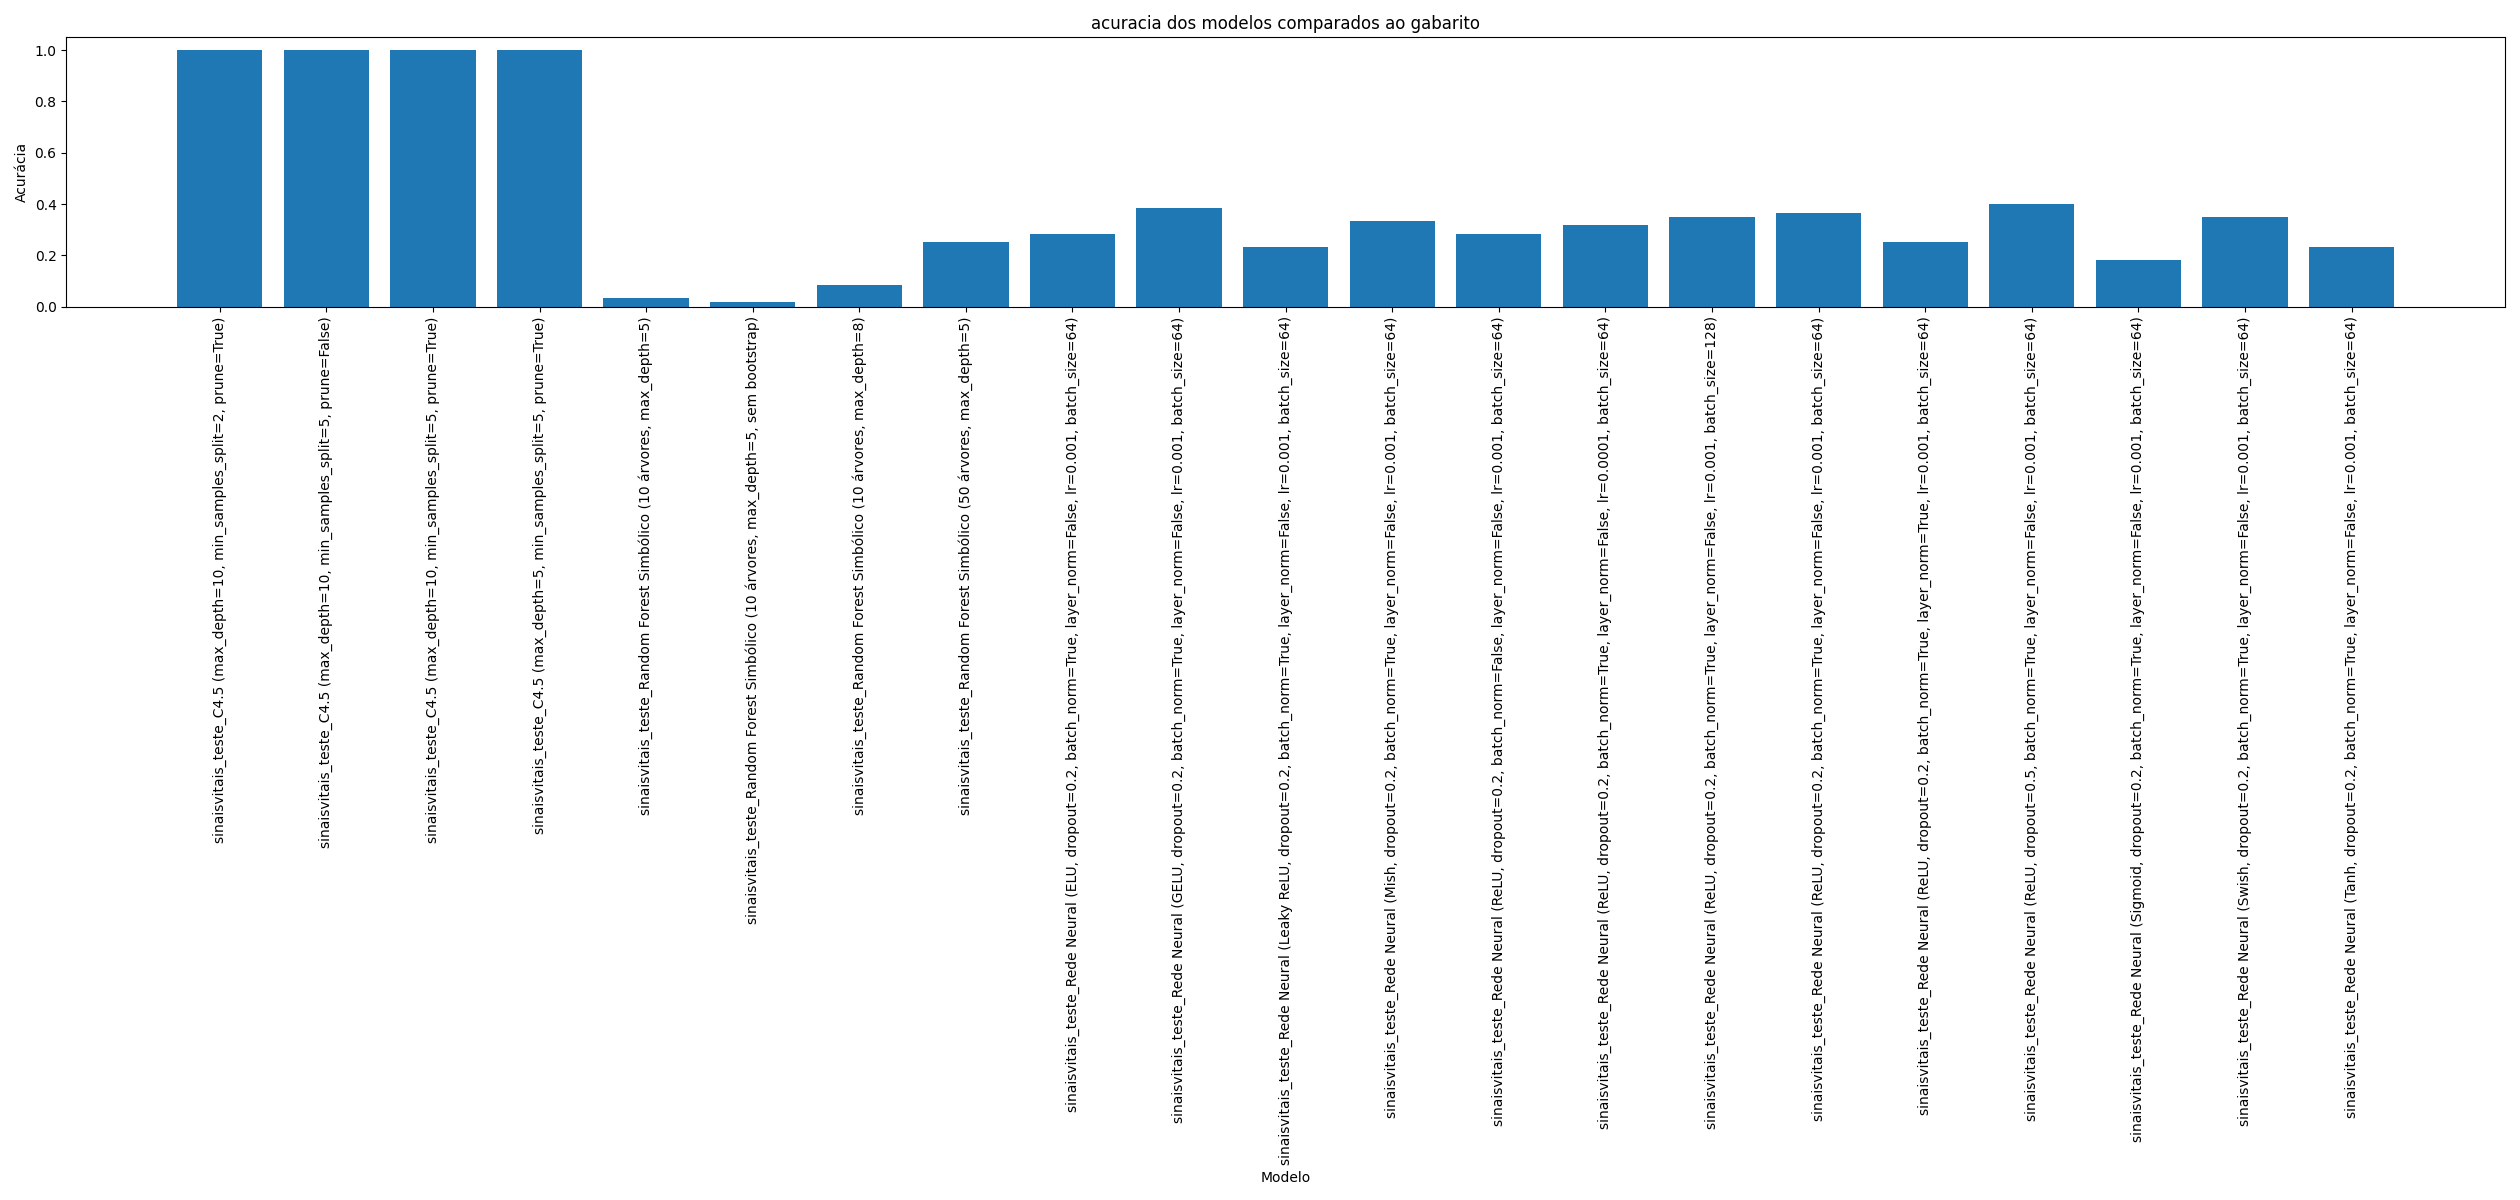
\includegraphics[width=0.7\textwidth]{comparacao_acuracia.png}
\caption{Comparação da acurácia entre os modelos avaliados.}
\label{fig:comparacao_acuracia}
\end{figure}

\begin{figure}[ht]
\centering
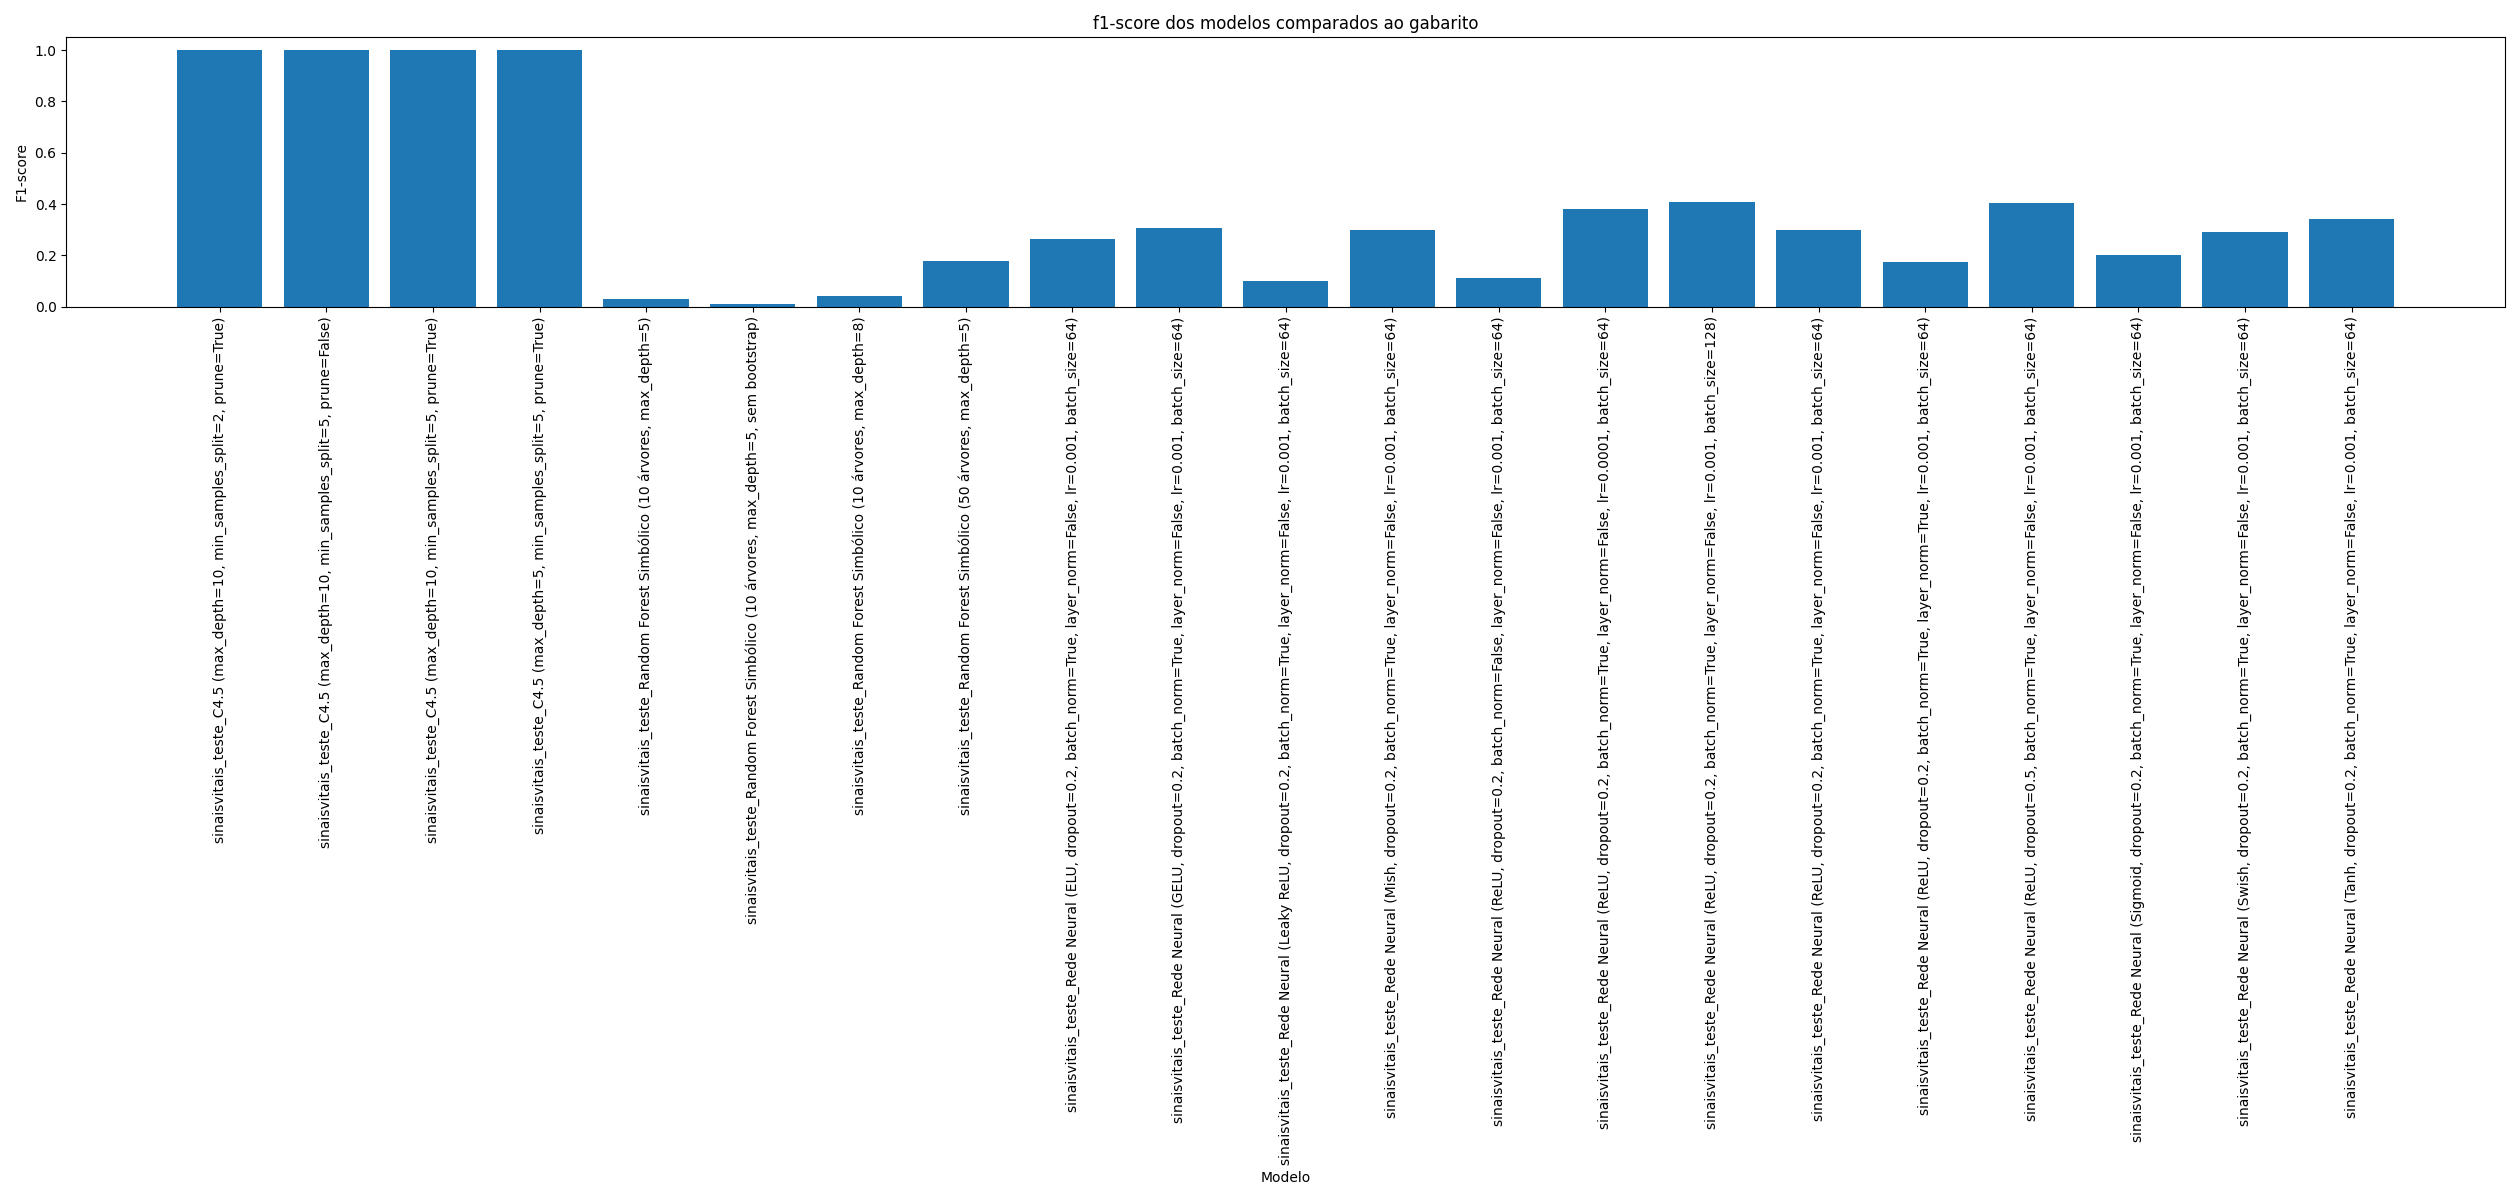
\includegraphics[width=0.7\textwidth]{comparacao_f1-score.png}
\caption{Comparação do F1-score entre os modelos avaliados.}
\label{fig:comparacao_f1}
\end{figure}

\begin{figure}[ht]
\centering
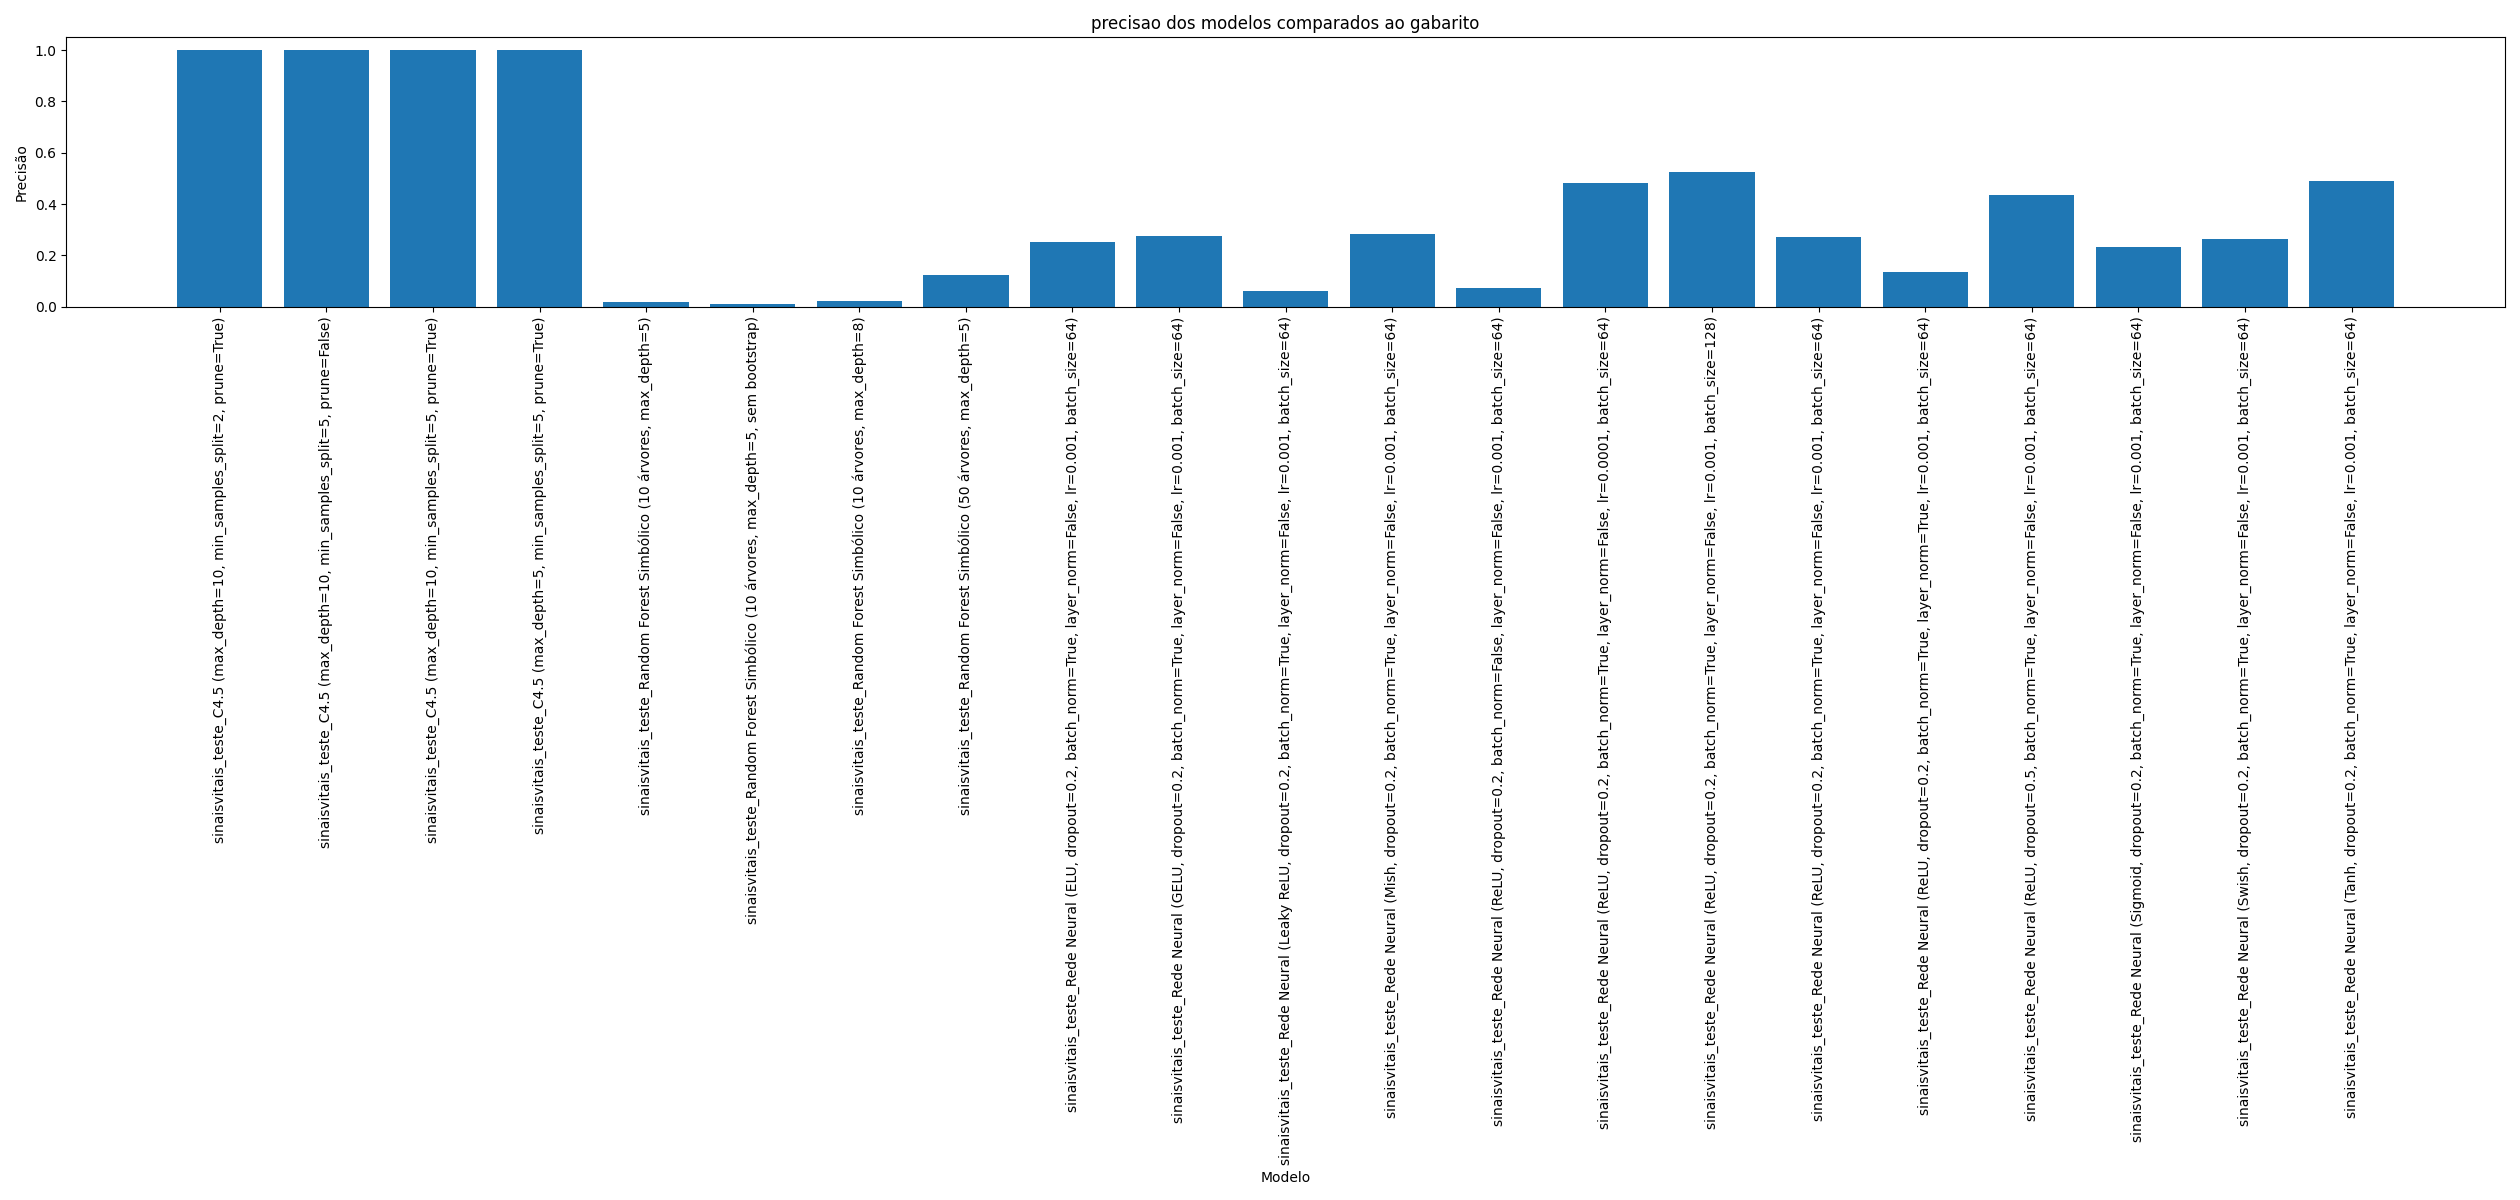
\includegraphics[width=0.7\textwidth]{comparacao_precisao.png}
\caption{Comparação da precisão entre os modelos avaliados.}
\label{fig:comparacao_precision}
\end{figure}

\begin{figure}[ht]
\centering
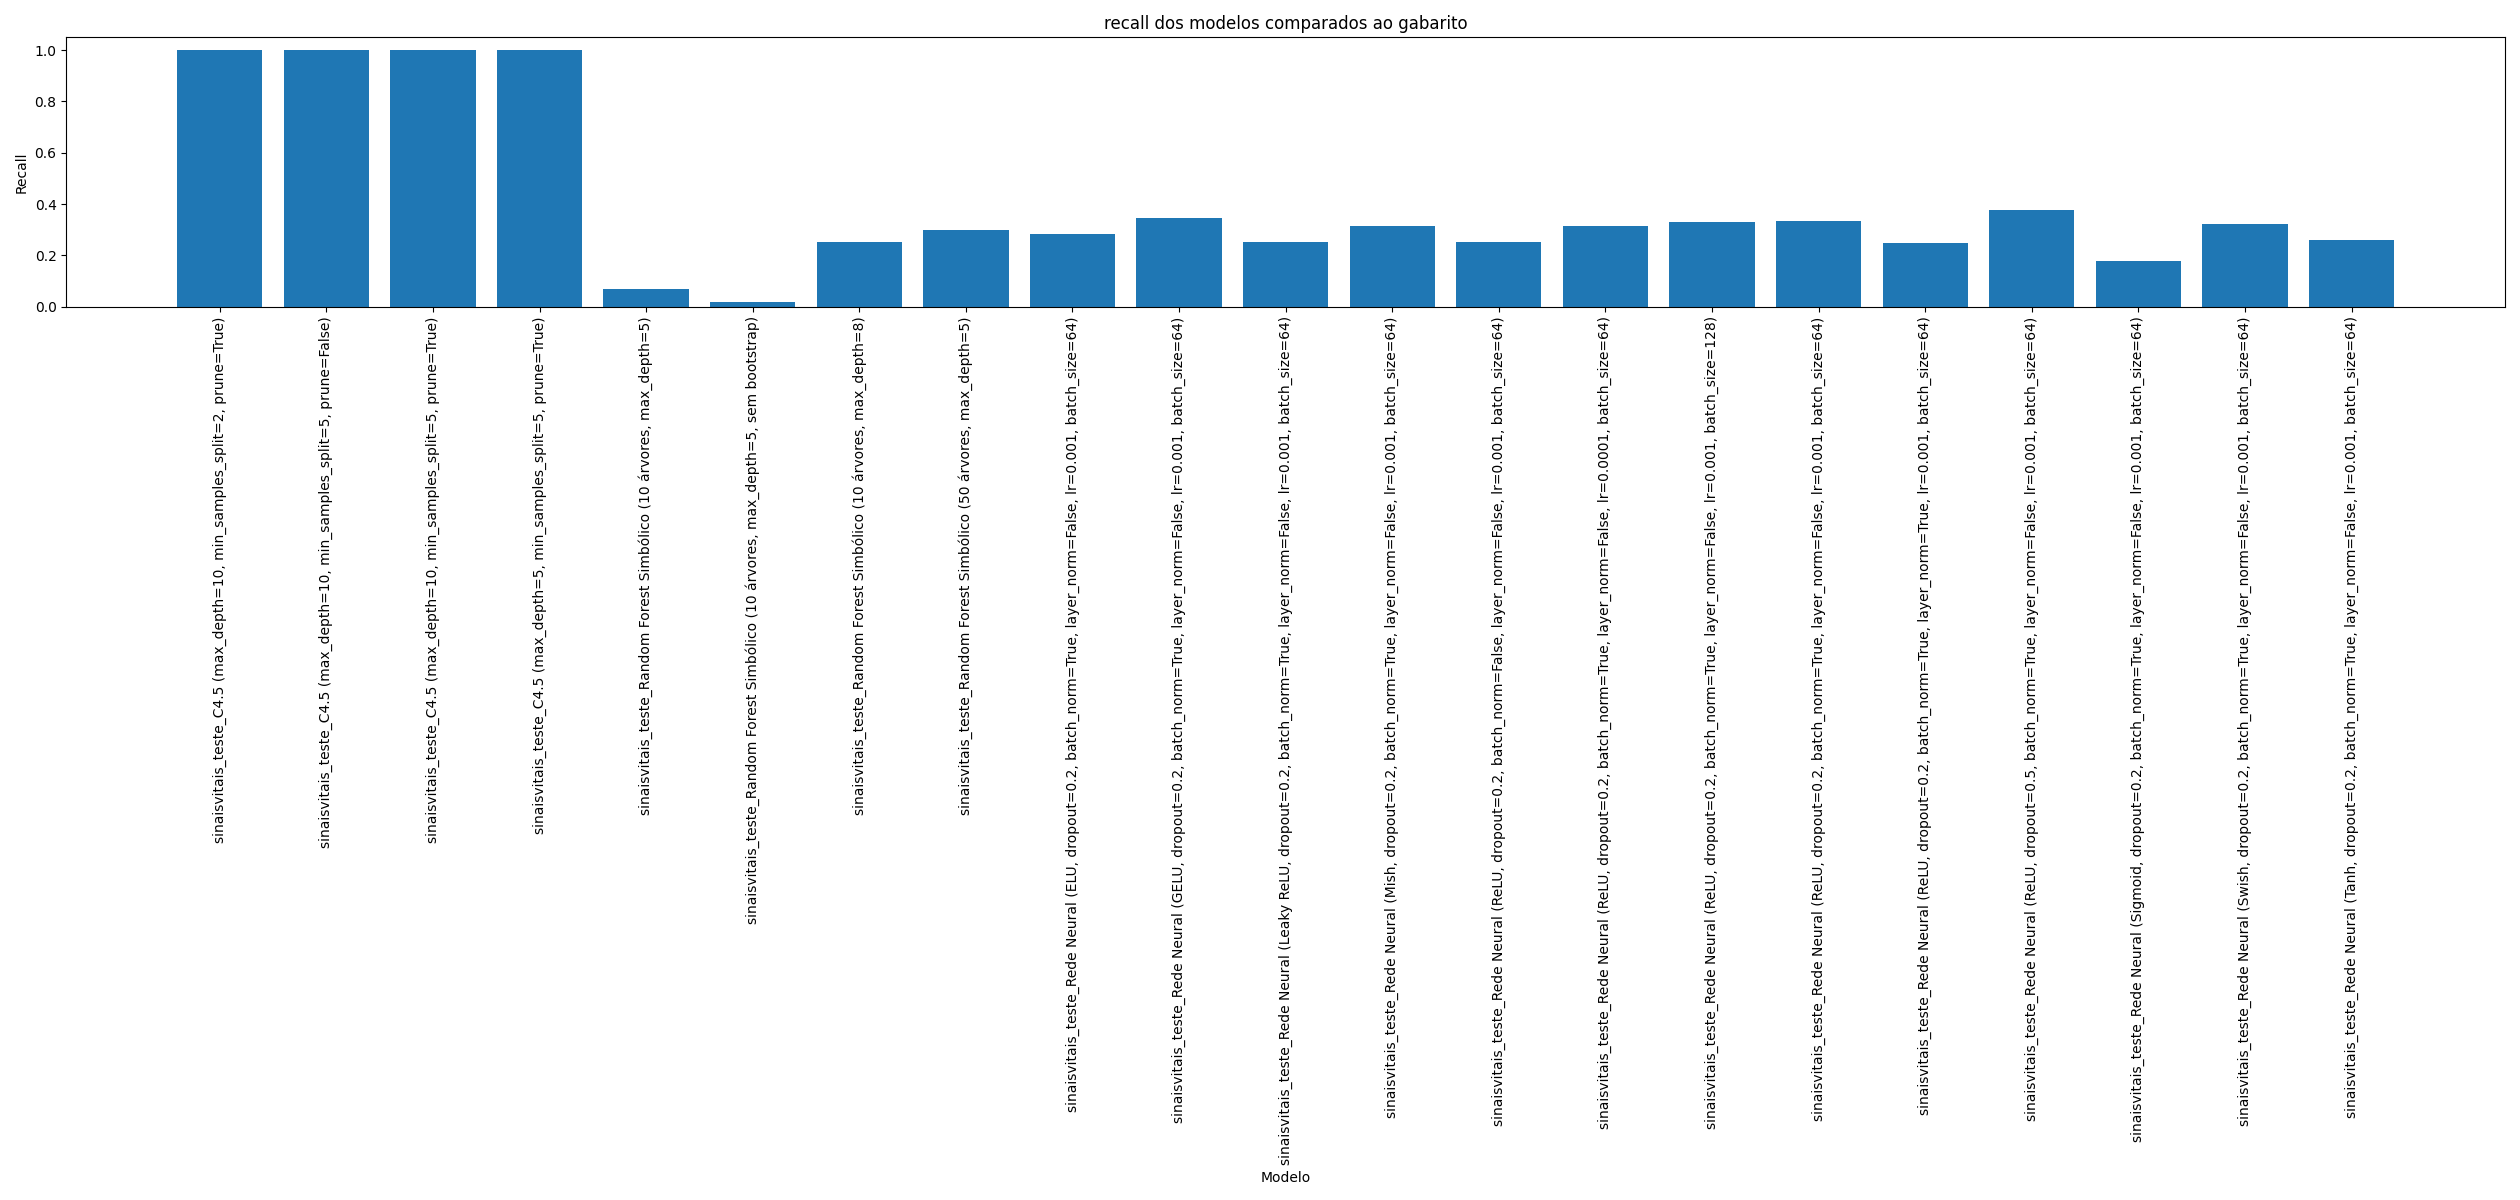
\includegraphics[width=0.7\textwidth]{comparacao_recall.png}
\caption{Comparação do recall entre os modelos avaliados.}
\label{fig:comparacao_recall}
\end{figure}

\begin{figure}[ht]
\centering
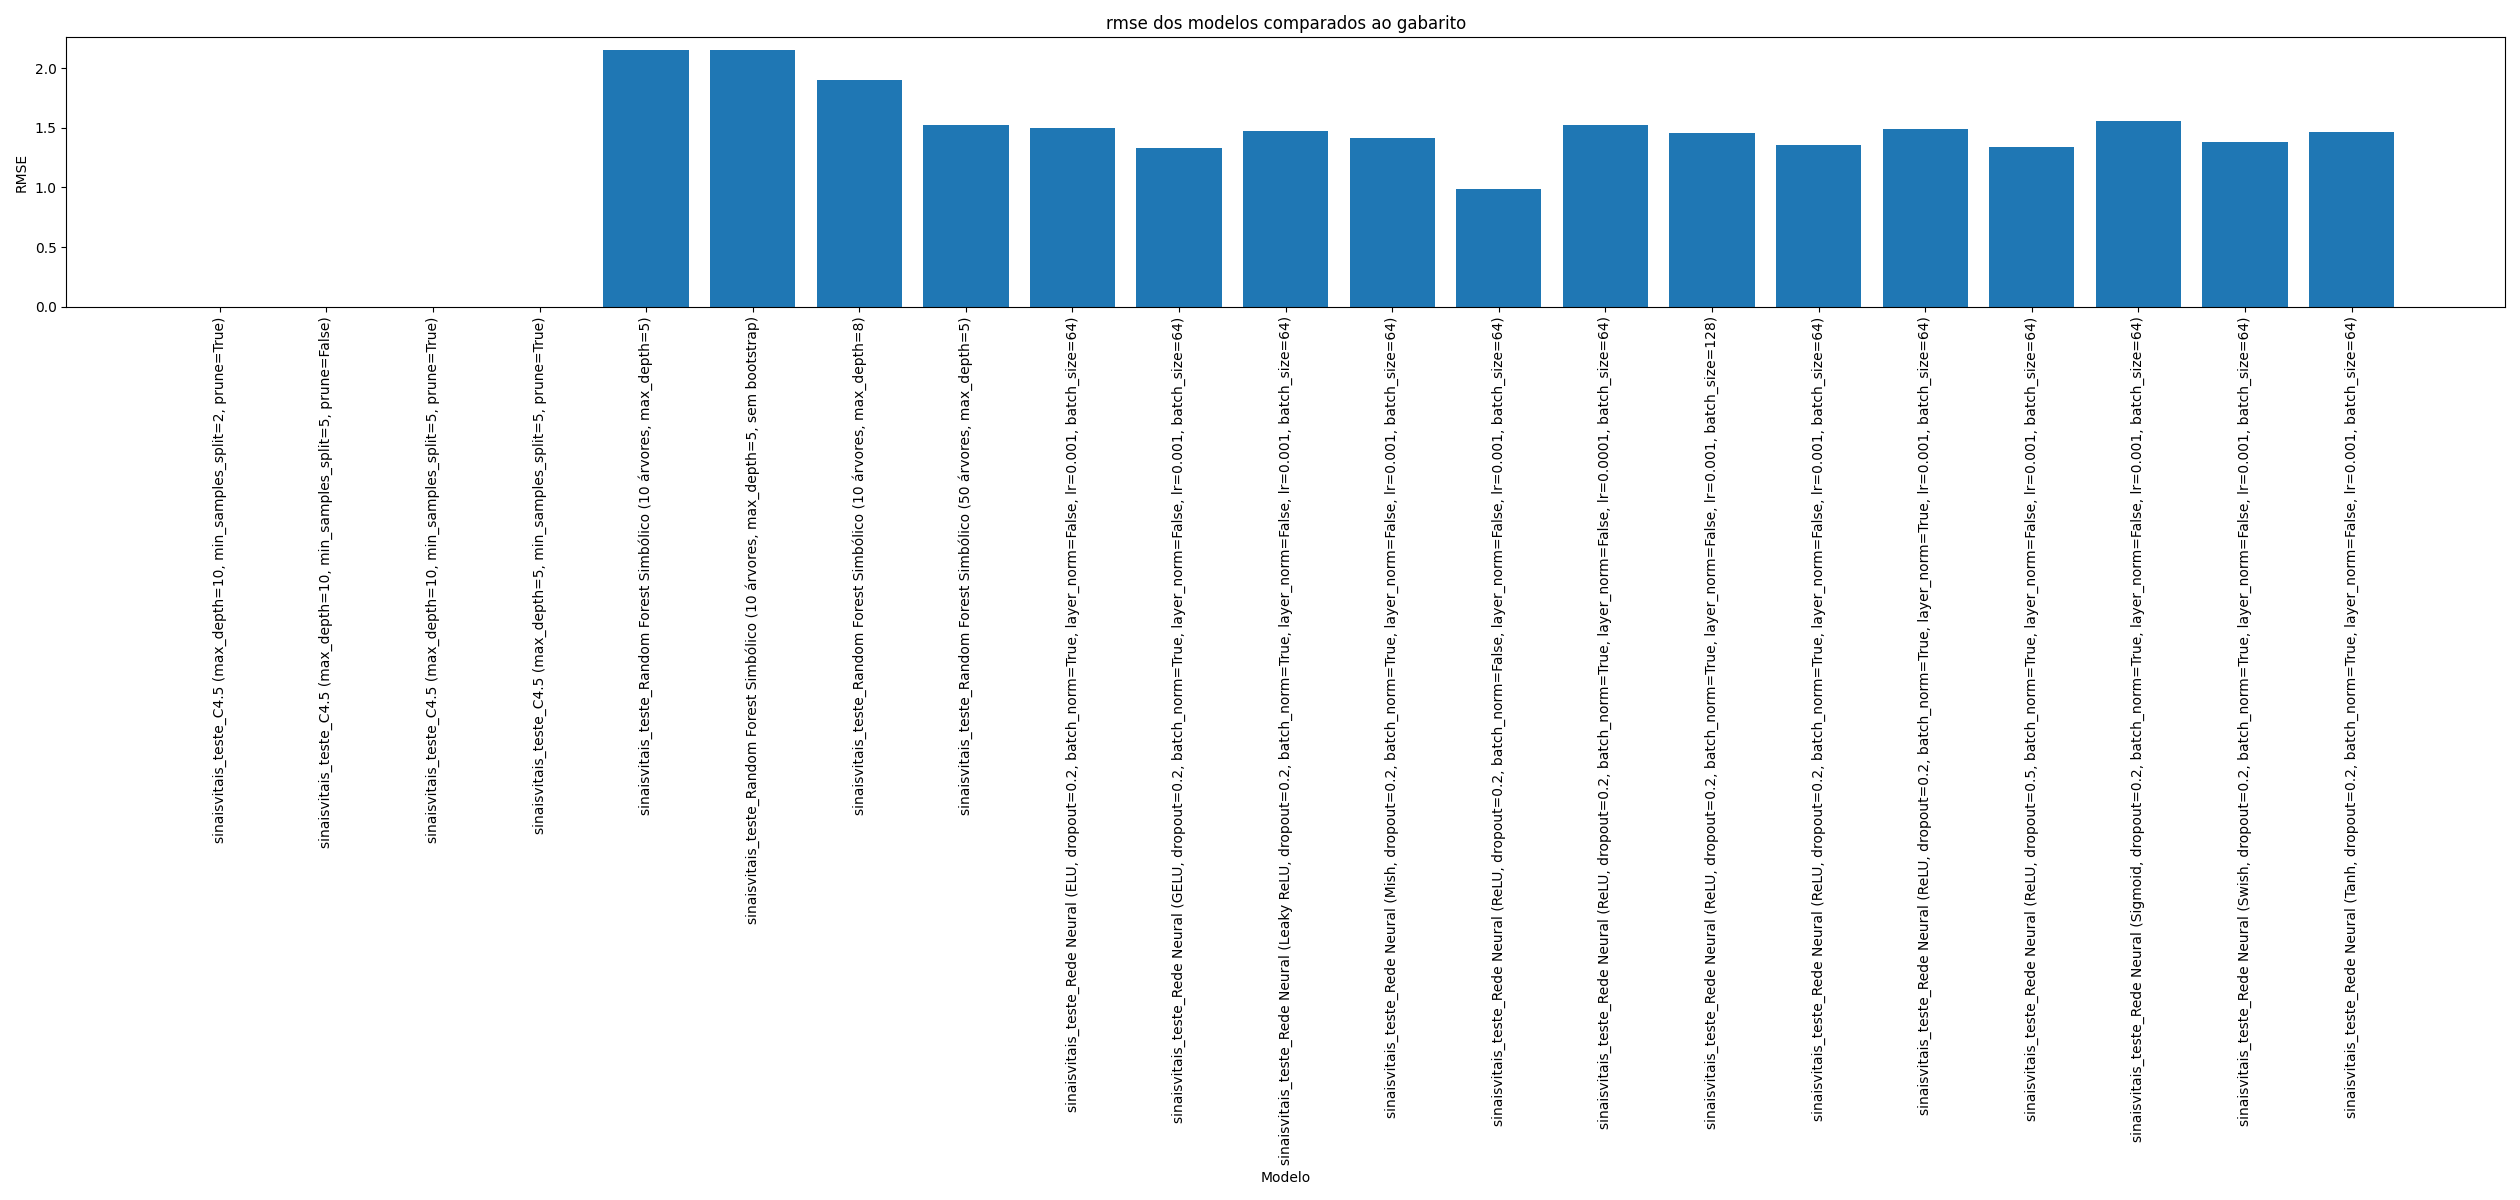
\includegraphics[width=0.7\textwidth]{comparacao_rmse.png}
\caption{Comparação do RMSE entre os modelos avaliados.}
\label{fig:comparacao_rmse}
\end{figure}

\section{Pseudocódigos dos Algoritmos}
\subsection{Random Forest Simbólico}
\begin{algorithm}[H]
\caption{Random Forest Simbólico}
\begin{algorithmic}[1]
\Procedure{TrainSymbolicRF}{$X, y, N, d_{max}$}
    \State Inicializar lista de árvores vazia
    \For{$i = 1$ até $N$}
        \State $X_i, y_i \gets$ bootstrap($X, y$)
        \State $tree_i \gets$ BuildSymbolicTree($X_i, y_i, d_{max}$)
        \State Adicionar $tree_i$ à lista de árvores
    \EndFor
    \State \Return lista de árvores treinadas
\EndProcedure
\Procedure{PredictSymbolicRF}{$X, \{tree_1, ..., tree_N\}$}
    \State Inicializar lista de predições vazia
    \For{cada $tree_i$ na lista de árvores}
        \State $pred_i \gets tree_i.predict(X)$
        \State Adicionar $pred_i$ à lista de predições
    \EndFor
    \If{tarefa é regressão}
        \State \Return média das predições para cada teste
    \Else
        \State \Return voto majoritário das predições para cada teste
    \EndIf
\EndProcedure
\end{algorithmic}
\end{algorithm}

\subsection{C4.5}
\begin{algorithm}[H]
\caption{C4.5}
\begin{algorithmic}[1]
\Procedure{TrainC45}{$X, y$}
    \If{todas as amostras têm o mesmo rótulo}
        \State \Return folha com esse rótulo
    \EndIf
    \For{cada atributo}
        \State calcular gain ratio para possíveis splits
    \EndFor
    \State selecionar melhor atributo e threshold
    \State dividir dados em dois subconjuntos
    \State recursivamente construir subárvores para cada subconjunto
    \State realizar poda se necessário
    \State \Return árvore construída
\EndProcedure
\Procedure{PredictC45}{árvore, $X$}
    \For{cada exemplo $x$ em $X$}
        \State percorrer a árvore a partir da raiz
        \While{nó não for folha}
            \State verificar valor do atributo no nó atual
            \State seguir para o ramo correspondente
        \EndWhile
        \State atribuir rótulo da folha ao exemplo $x$
    \EndFor
    \State \Return rótulos preditos
\EndProcedure
\end{algorithmic}
\end{algorithm}

\subsection{Perceptron Multicamadas (MLP)}
\begin{algorithm}[H]
\caption{Perceptron Multicamadas (MLP)}
\begin{algorithmic}[1]
\Procedure{TrainMLP}{$X, y, \theta$}
    \State Inicializar pesos $W_l$ e biases $b_l$ para cada camada $l$
    \For{época = 1 até max\_epochs}
        \For{cada batch $(X_{batch}, y_{batch})$ em $X, y$}
            \State $a_0 \gets X_{batch}$
            \For{camada $l = 1$ até $L$}
                \State $z_l \gets a_{l-1} W_l + b_l$
                \State $a_l \gets$ ativação($z_l$)
                \If{dropout}
                    \State aplicar máscara de dropout em $a_l$
                \EndIf
            \EndFor
            \State $loss \gets$ calcular\_erro($a_L, y_{batch}$)
            \State backpropagation($loss$) para obter gradientes de $W_l, b_l$
            \State atualizar $W_l, b_l$ com gradiente descendente
        \EndFor
        \If{early stopping com base na validação}
            \State parar treinamento
        \EndIf
    \EndFor
\EndProcedure
\Procedure{PredictMLP}{$X$}
    \State $a_0 \gets X$
    \For{camada $l = 1$ até $L$}
        \State $z_l \gets a_{l-1} W_l + b_l$
        \State $a_l \gets$ ativação($z_l$)
    \EndFor
    \State \Return $a_L$ (saída da rede)
\EndProcedure
\end{algorithmic}
\end{algorithm}

\section{Figuras Ilustrativas dos Algoritmos}

\subsection{Árvore de Decisão (Exemplo)}
\begin{figure}[ht]
\centering
\begin{forest}
for tree={
    draw,
    rounded corners,
    node options={align=center},
    s sep=10mm,
    l sep=10mm
}
[Raiz: $x_1 > 0.5$?
    [Sim\\$x_2 > 0.3$?
        [Classe 1]
        [Classe 2]
    ]
    [Não
        [Classe 3]
    ]
]
\end{forest}
\caption{Exemplo de árvore de decisão binária.}
\end{figure}

\subsection{Perceptron Simples}
\begin{figure}[ht]
\centering
\begin{tikzpicture}[scale=1.2]
% Entradas
\foreach \i in {1,2,3}
    \node[circle,draw,minimum size=0.7cm] (x\i) at (0,-\i) {$x_{\i}$};
% Neurônio
\node[circle,draw,minimum size=1cm,fill=gray!10] (n) at (2,-2) {$\sum$};
% Pesos
\foreach \i in {1,2,3}
    \draw[->] (x\i) -- (n);
% Saída
\draw[->] (n) -- ++(1.2,0) node[right] {$y = \phi(\sum w_i x_i + b)$};
\end{tikzpicture}
\caption{Diagrama de um perceptron simples.}
\end{figure}

\subsection{Perceptron Multicamadas (MLP)}
\begin{figure}[ht]
\centering
\begin{tikzpicture}[scale=1.1, every node/.style={scale=0.9}]
% Camada de entrada
\foreach \i in {1,...,3}
    \node[circle,draw,minimum size=0.7cm] (I\i) at (0,-\i) {$x_{\i}$};
% Camada oculta
\foreach \i in {1,...,4}
    \node[circle,draw,minimum size=0.7cm,fill=blue!10] (H\i) at (2,-0.5-\i) {};
% Camada de saída
\node[circle,draw,minimum size=0.7cm,fill=red!10] (O) at (4,-2.5) {$y$};
% Conexões
\foreach \i in {1,...,3}
    \foreach \j in {1,...,4}
        \draw[->] (I\i) -- (H\j);
\foreach \j in {1,...,4}
    \draw[->] (H\j) -- (O);
\end{tikzpicture}
\caption{Exemplo de Perceptron Multicamadas (MLP) com 3 entradas, 1 camada oculta e 1 saída.}
\end{figure}

\subsection{Representação de Tensor (Matriz 3D)}
\begin{figure}[ht]
\centering
\begin{tikzpicture}[scale=1.2]
% Eixos
\draw[->] (0,0,0) -- (2.2,0,0) node[right] {$x$};
\draw[->] (0,0,0) -- (0,2.2,0) node[above] {$y$};
\draw[->] (0,0,0) -- (0,0,2.2) node[left] {$z$};
% Pontos da matriz 3D
\foreach \x in {0,1}
  \foreach \y in {0,1}
    \foreach \z in {0,1}
      \filldraw[blue] (\x,\y,\z) circle (1.5pt);
% Linhas para formar o cubo
\draw[thick] (0,0,0) -- (1,0,0) -- (1,1,0) -- (0,1,0) -- cycle;
\draw[thick] (0,0,1) -- (1,0,1) -- (1,1,1) -- (0,1,1) -- cycle;
\draw[thick] (0,0,0) -- (0,0,1);
\draw[thick] (1,0,0) -- (1,0,1);
\draw[thick] (1,1,0) -- (1,1,1);
\draw[thick] (0,1,0) -- (0,1,1);
% Números
\node at (0,0,0) [below left] {\small $a_{000}$};
\node at (1,0,0) [below right] {\small $a_{100}$};
\node at (0,1,0) [above left] {\small $a_{010}$};
\node at (1,1,0) [above right] {\small $a_{110}$};
\node at (0,0,1) [below left] {\small $a_{001}$};
\node at (1,0,1) [below right] {\small $a_{101}$};
\node at (0,1,1) [above left] {\small $a_{011}$};
\node at (1,1,1) [above right] {\small $a_{111}$};
\end{tikzpicture}
\caption{Representação de uma matriz tridimensional (tensor 3D) com índices explícitos.}
\end{figure}

\end{document}
